%
% 講演資料
%  https://scrapbox.io/masui/ソフトウェア科学会_基礎研究賞講演_2021/9/3
% Cloud LaTeX
%  https://cloudlatex.io/projects/411855/edit
% 記事依頼
%  https://mail.google.com/mail/u/0/?zx=a0kk8p4fqhm3#inbox/WhctKKWxdNgXpJNJdpfrtHgVMQJTthSKpCLwgCTppBnkqJbWZmmsxwzHgMwmjcxmLrKmfZV
% 執筆要項 (スタイルファイル)
%  https://www.jssst.or.jp/edit/detail/style_files.html
% 記事例
%  https://s3-ap-northeast-1.amazonaws.com/masui.org/f/5/f5361cf93c65dd661e5797ed105bfeca.pdf
%

\long\def\comment#1{}

\documentclass[topics]{compsoft} % トピックス


% 「コンピュータソフトウェア」誌に掲載される論文の場合,次で巻数,号数,開始ページ,終了ページを指定する.
\volNoPp{39}{1}{1}{6}

% \usepackage[dvips]{graphics}

\usepackage{graphicx}

\usepackage{here} % [H]とするとその場所に配置されるらしい

\begin{document}

\title{ユニバーサルなユーザインタフェース}

% 著者
% 和文論文の場合,姓と名の間には半角スペースを入れ,
% 複数の著者の間は全角スペースで区切る
%
\author{増井 俊之
%
% ここにタイトル英訳 (英文の場合は和訳) を書く.
%
\ejtitle{Universal user interfaces.}
%
% ここに著者英文表記 (英文の場合は和文表記) および
% 所属 (和文および英文) を書く.
% 複数著者の所属はまとめてよい.
%
\shozoku{Toshiyuki Masui}{慶應義塾大学 環境情報学部}%
{Faculty of Environment and Information Studies, Keio University}
%
% 出典情報は \shutten とすれば出力される.
\shutten
%
% 受付年月日,記事カテゴリなどは自動的に生成される.
\uketsuke{2021}{11}{15}
%
% その他,脚注に入れるものがあれば,\note に記述する.
%\note{脚注に入れる内容}
}

% 和文アブストラクト
\Jabstract{%
ユーザインタフェースとは
}
%
% 英文アブストラクト(本サンプルの原論文にはなし)
\Eabstract{%
We talk ablut uniersal UI.
%
}

\maketitle

\section{はじめに}

私は30年以上にわたり、コンピュータの使いやすさを改善する
ユーザインタフェースの研究開発を行なってきました。
このことが評価され、2020年度日本ソフトウェア科学会基礎研究賞を頂くことができ、
大変光栄に思っております。
受賞業績のタイトルである「ユニバーサルなユーザインタフェース」について、
世の中の動向および私自身の研究について紹介させていただきます。

昔のコンピュータは専門家が使うものでしたが、
最近は誰もががパソコンやスマホでコンピュータやインターネットを活用しています。
これはコンピュータのユーザインタフェースの改良の結果です。

コンピュータが世の中で使われはじめた頃は
文字ベースの入出力(Command Line Interface: CLI)が一般的でしたが、
1970年代に高解像度ディスプレイの上の
ウィンドウやメニューなどを利用する
グラフィカルユーザインタフェース(Graphical User Interface: GUI)がXerox PARC\footnote{
  \textsf{https:{\slash}{\slash}ja.wikipedia.org{\slash}wiki{\slash}パロアルト研究所}
}で発明されて以来コンピュータ利用のハードルが低くなり、
現在は多くの人々がコンピュータを使えるようになりました。

近年のコンピュータ利用のトレンドを表現するキーワードとして
「モバイルコンピューティング」や「ユビキタスコンピューティング」といったものがあります。
これらの言葉には、
コンピュータを誰もがいつでも使うというニュアンスがあり、
コンピュータが「ユニバーサル」に使えるようになってきたことのあらわれでしょう。
%
「ユニバーサル」というのは、
障害や年齢などにかかわらず「誰でも使える」という意味です。
例えば、体が多少不自由でも言葉が通じなくても「自動ドア」を使うことができますから、
自動ドアはユニバーサルに利用できるインタフェースだといえます。
%
誰でも使えるユニバーサルなシステムの設計は
「ユニバーサルデザイン」と呼ばれ、
この考え方の重要性が広く認識されるようになってきました。

\comment{
ユニバーサルデザインの考え方はコンピュータに限ったものではありません。
最近建築される家屋は段差が無いように設計されているものが多く、
歩行が得意でない人間でも生活しやすいようになっていますが、
これは建築におけるユニバーサルデザインです。
%
家の中の段差などは誰にとっても邪魔なものであり、
こういう問題を解決するための
ユニバーサルデザインはあらゆる人にとって有益なはずです。
}

% 特定の障害を念頭に置かず、
% 常にあらゆる人が利用できるシステムを設計することが重要だということが認識されてきたように思われます。

\comment{
これまでのコンピュータは
高度な計算、大量の記憶、コミュニケーションのサポート、情報入力/編集のサポート、
情報検索のサポートなど様々な用途に利用されてきましたが、
おおざっぱに言うと、
コンピュータは「人間の弱点を補強する」ために広く利用されてきたということができるかもしれません。

以前は専門家の仕事を補助するために、
また現在は一般人が苦手としていることを助けるために、
人々の弱点を補強する用途として利用されているわけです。
将来は、さらに広い領域で人々をサポートするために
コンピュータが使われることがもっと増えてくることでしょう。
}

近年、「Augmented Human」というキーワードで
研究が行なわれたりコンファレンスが開かれたりしています\footnote{
  \textsf{https:{\slash}{\slash}www.augmented-human.com{\slash}}
}。
これは「人間の能力をコンピュータで拡張する」というコンセプトを表現する言葉ですが、
様々な技術で人を助けたり能力を増強したりするという考えは新しいものではありません。
服もメガネも自動車も文房具も、
すべて人間の能力を拡張するためのものであり、
これらは大きな産業になっています。

私がユーザインタフェースの研究をはじめた1980年代は
コンピュータは専門家が使うものだと考えられており、
誰もが使えるコンピュータを作るといった考えはポピュラーではありませんでした。
%
しかし現在は誰もがパソコンやスマホを活用していますし、
将来はユニバーサルデザインという考え方にもとづいて、
あらゆる人間の弱点を補強したり能力を拡張したりする用途に
コンピュータがより広く利用されるようになるでしょう。

\section{ユニバーサルなシステム開発例}

私はユニバーサルであることを重視した
様々なインタフェースシステムを開発したり普及を試みたりしてきました。
そのようなシステムの実例をいくつか紹介します。

\subsection{テキスト入力支援}

私は2000年ごろ、
当時普及しつつあった携帯電話のための
予測型日本語入力手法「POBox」\footnote{
  \textsf{https:{\slash}{\slash}ja.wikipedia.org{\slash}wiki{\slash}POBox}
}を製品化しました。

\begin{figure}[h]
  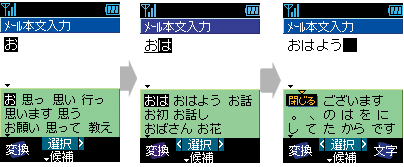
\includegraphics[width=10cm,bb=0 0 404 167]{figures/ac2b347a7042f920edd576ee07c4b7f4.png}
  \caption{auの携帯電話に登載されたPOBox.}
  \label{pobox}
\end{figure}

コンピュータが人間の操作を予測することにより
人間の操作の手間を減らす「予測インタフェース」システムの研究が
従来から行なわれていましたが\cite{WatchWhatIDo}\cite{YourWish}、
POBoxはこれをテキスト入力に応用したものです。
%
POBoxは、携帯電話での商品化以前に、
携帯端末PalmPilot\footnote{
  \textsf{https:{\slash}{\slash}ja.wikipedia.org{\slash}wiki{\slash}PalmPilot}
}上に実装したものが
PalmPilotユーザの間では広く利用されていましたが、
携帯電話上で利用できるようになったために
多くの携帯電話ユーザが利用するようになりました。
この結果、
予測型入力システムは、小型のモバイル機器での
テキスト入力に便利だということが広く認知され、
現在は携帯機器でのテキスト入力手法の実質的な標準となっています。

テキスト入力に予測インタフェースを利用するという手法は、
手が不自由なユーザのための特殊な入力インタフェースとして
従来から利用されていましたが、
POBoxは、誰もが使えるユニバーサルなインタフェースとしてデザインされ普及したところに意義があります。
ユニバーサルなユーザインタフェースの工夫によって、
あらゆる人々が使えるシステムを作ることが可能になることを示せたといえるでしょう。

\begin{figure}[h]
  \centerline{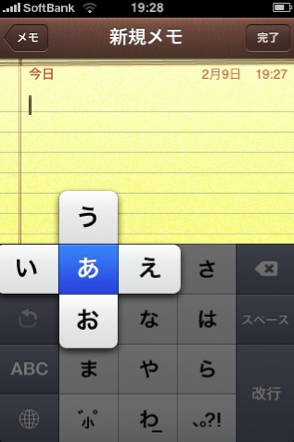
\includegraphics[width=6cm,bb=0 0 294 442]{figures/1691febad27439d3bf44232c54dcb1e8.png}}
  \caption{iPhoneのフリック入力.}
  \label{flick}
\end{figure}

現在、予測型テキスト入力手法は
スマホのような機器の入力手法として広く利用されていますが、
手が不自由な人のための入力システムPETE\footnote{
  \textsf{https:{\slash}{\slash}www.ideafront.jp{\slash}PeteHP{\slash}}
}などでも利用されています。
PETEでは、キーボードをタップすることによって
入力単語の読みを入力するのではなく、
キーボードの行や列の上を移動するカーソルが
目的の文字の上に来たタイミングでボタンを押すことによって読みを指定します。
このため、キーボードをタップすることができないユーザでも
単語の読みからテキスト入力を行なうことができます。

\begin{figure}[h]
  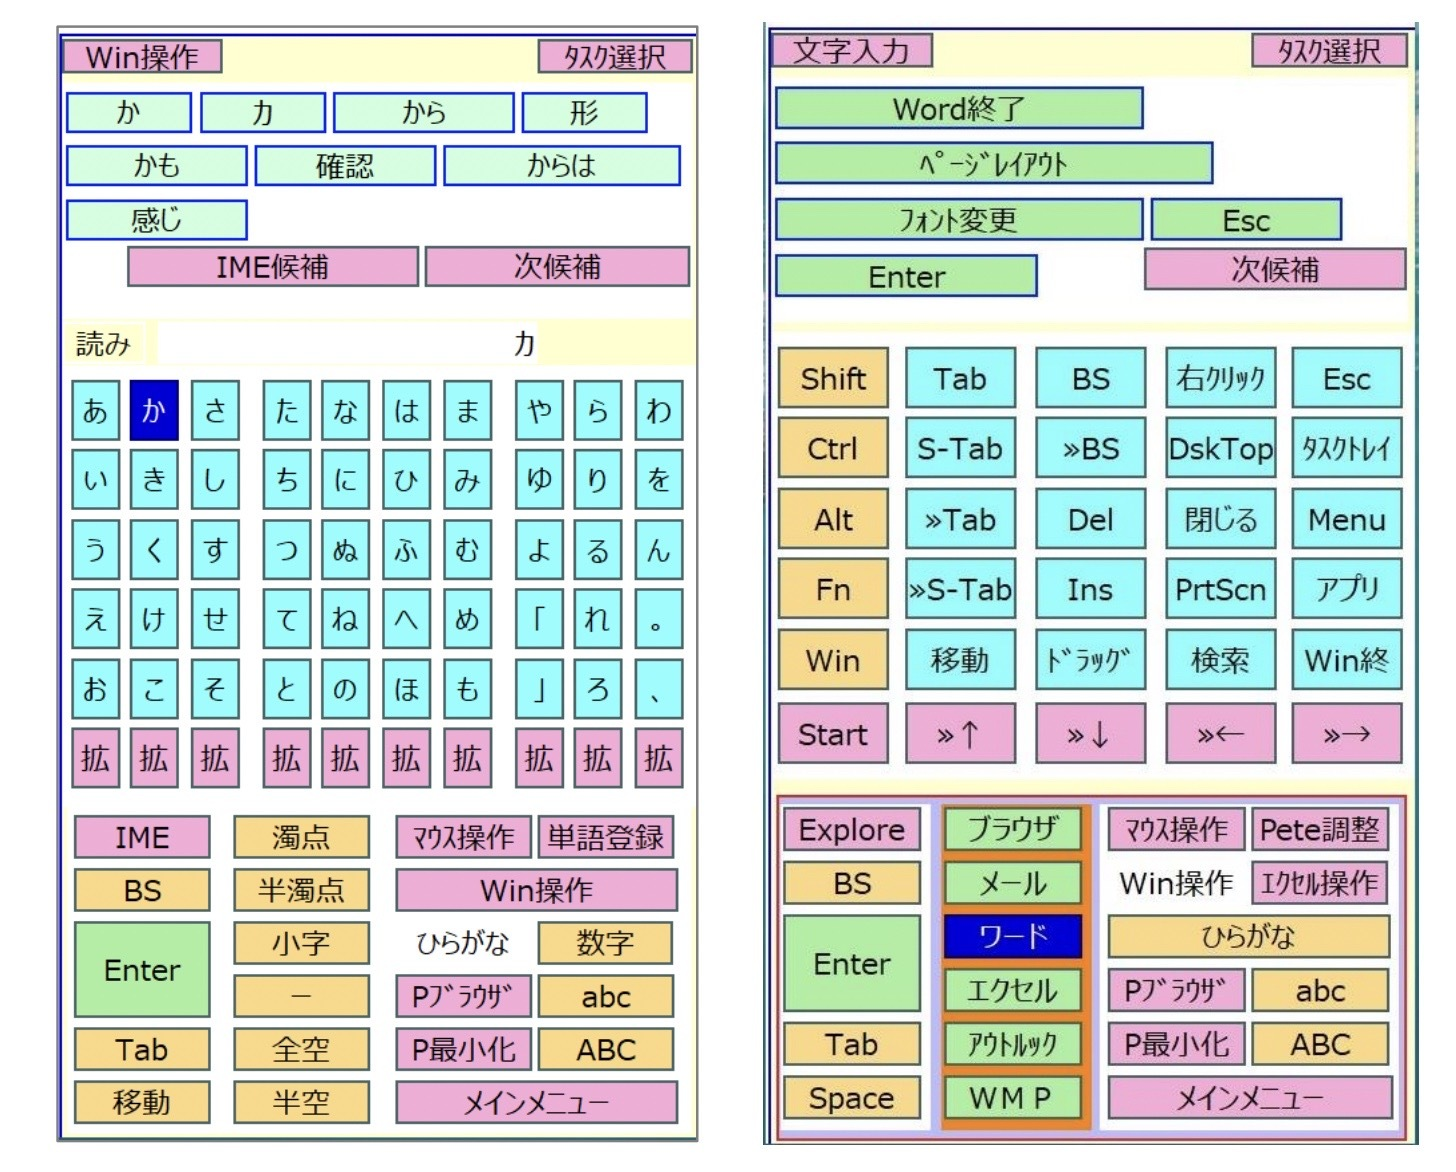
\includegraphics[width=10cm,bb=0 0 1456 1172]{figures/a2f652e2f488b96974e92f8198f49469.jpg}
  \caption{PETE利用画面.}
  \label{pete}
\end{figure}

\subsection{画面キャプチャ}

パソコンの画面の一部を切り出して
保存したり他人と共有したりしたいことがよくあります。
パソコンには画面をキャプチャして画像ファイルとして保存する機能がありますが、
キャプチャした画像をWebページで使ったり他人と共有したりすることは
意外と面倒でした。
この手間を省き、誰もが簡単に画像を共有できるようにするため、
画面上で領域を選択するとすぐにその画像がWeb上にアップロードされて固有のURLが付加される
「Gyazo」というソフトウェア\footnote{
  \textsf{https:{\slash}{\slash}Gyazo.com{\slash}}
}を2007年に開発して公開しました。

Gyazoを使うと単純な操作で画像を切り出して活用することができて便利なので、
ユーザが全世界で爆発的に増加し、
現在は月間1000万人のユーザがGyazoを利用しています。
%
Webのトラフィック情報を計測するAlexa\footnote{
  \textsf{https:{\slash}{\slash}www.alexa.com{\slash}}
}のデータによると、
Gyazoは全世界のWebサービスで数百番目にトラフィックが多いサービスになっています\footnote{
  世界で最もトラフィックが多いのはGoogle, 2番目はFacebook
}。

\begin{figure}[h]
  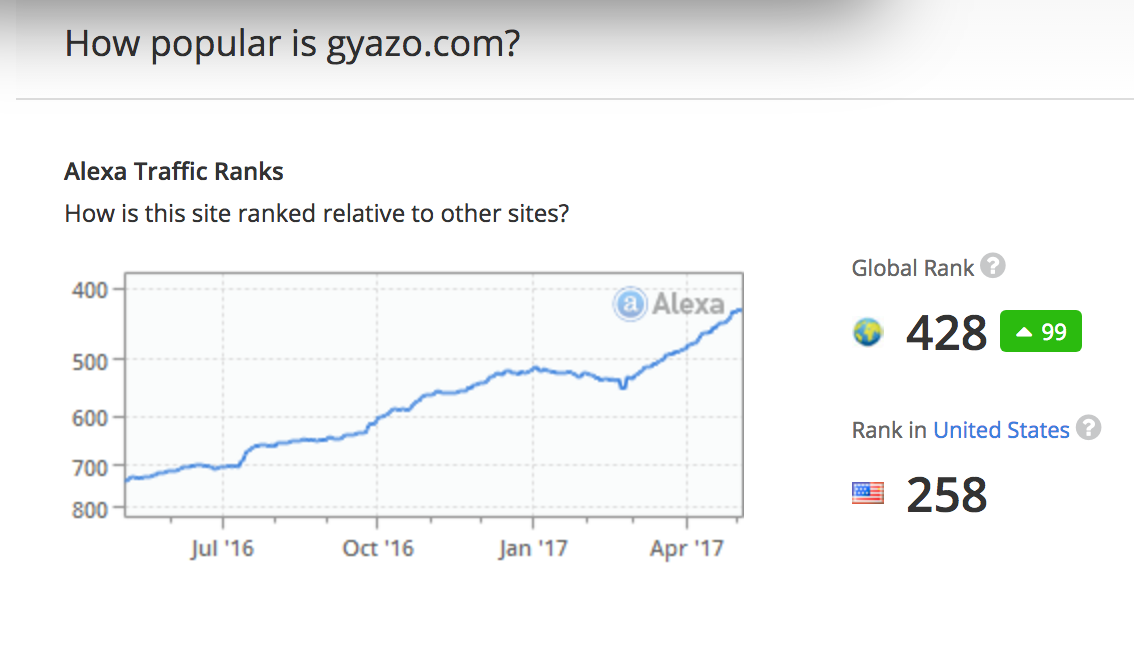
\includegraphics[width=10cm,bb=0 0 1134 668]{figures/2595e48e8346b423d6e6c1d23daf10f4.png}
  \caption{Gyazoのトラフィック.}
  \label{alexa}
\end{figure}

Gyazoでは画像キャプチャ時にアプリケーション情報などの付帯情報や
OCRテキストを記録するため、
画像をキャプチャするという簡単な操作だけで様々な情報整理を行なうこともできます。
面倒なことを考えなくても自動的に情報の整理が行なえるという点で、
Gyazoはユニバーサルなサービスであるといえるでしょう。

\subsection{思考支援}

アイデアをまとめたり文章を書いたりするのは努力が必要な作業です。
ワープロ、{\TeX}、HTMLなどを使ってコンピュータで美しい文章を作るのは一般的ですし、
アイデアや考えをまとめるための様々なシステムやサービスが提案されていますが、
決定版といえるものは存在しないので、
試行錯誤している人も多いでしょう。

私は、頭の中の考えをまとめたいときや情報を共有したいときは、
Wiki\footnote{
  \textsf{https:{\slash}{\slash}ja.wikipedia.org{\slash}wiki{\slash}ウィキ}
}を使うことが効果的だと考え、
Gyazz\cite{Gyazz}というシステムを作成して長年利用してきました。
現在は「Scrapbox」\footnote{
  \textsf{https:{\slash}{\slash}scrapbox.io{\slash}}
}という名前でサービス提供しています。

Scrapboxは、
ブラウザ上でリアルタイムに手軽に情報を共有することができるサービスです。
複数ユーザが同時にテキスト編集を行なえることに加え、
ページ間のリンクを簡単に作ることができるので、
様々な用途に使うことができます。

\begin{figure}[t]
  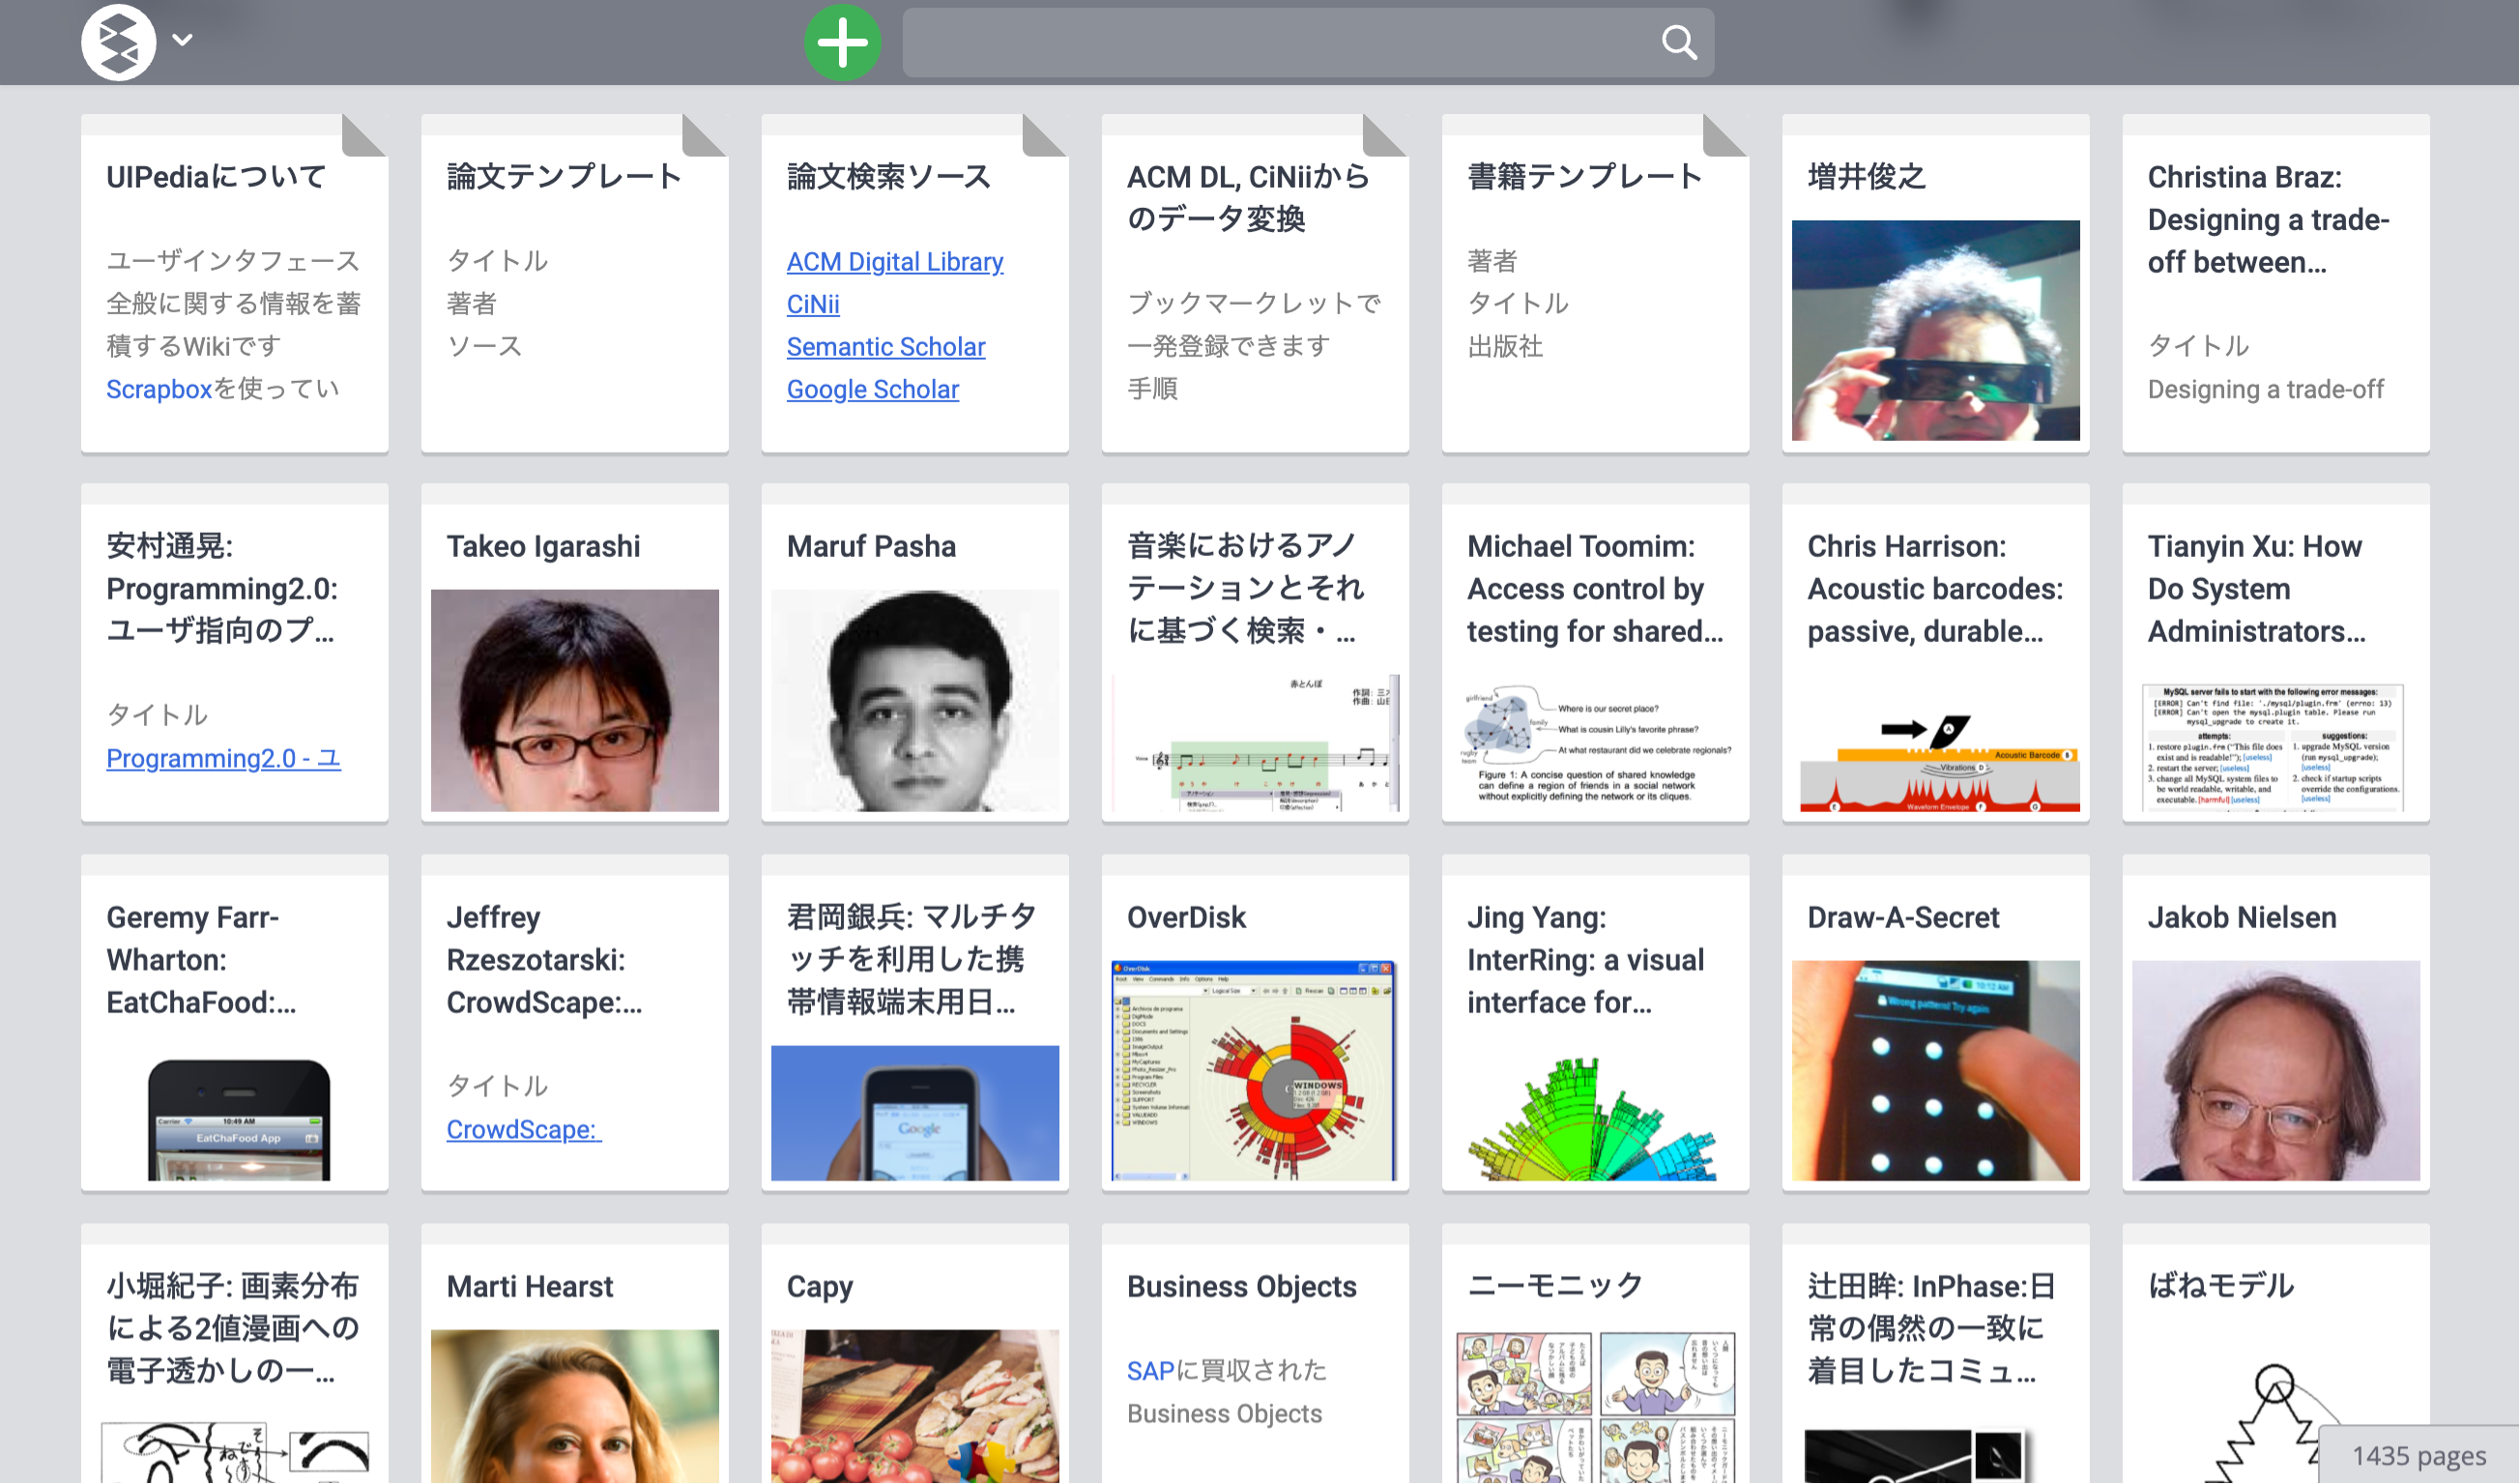
\includegraphics[width=9cm,bb=0 0 2607 1535]{figures/13982c755fdc0c60af2548c0a6589543.png}
  \caption{Scrapboxページのリスト.}
  \label{example1}
\end{figure}

\begin{figure}[t]
  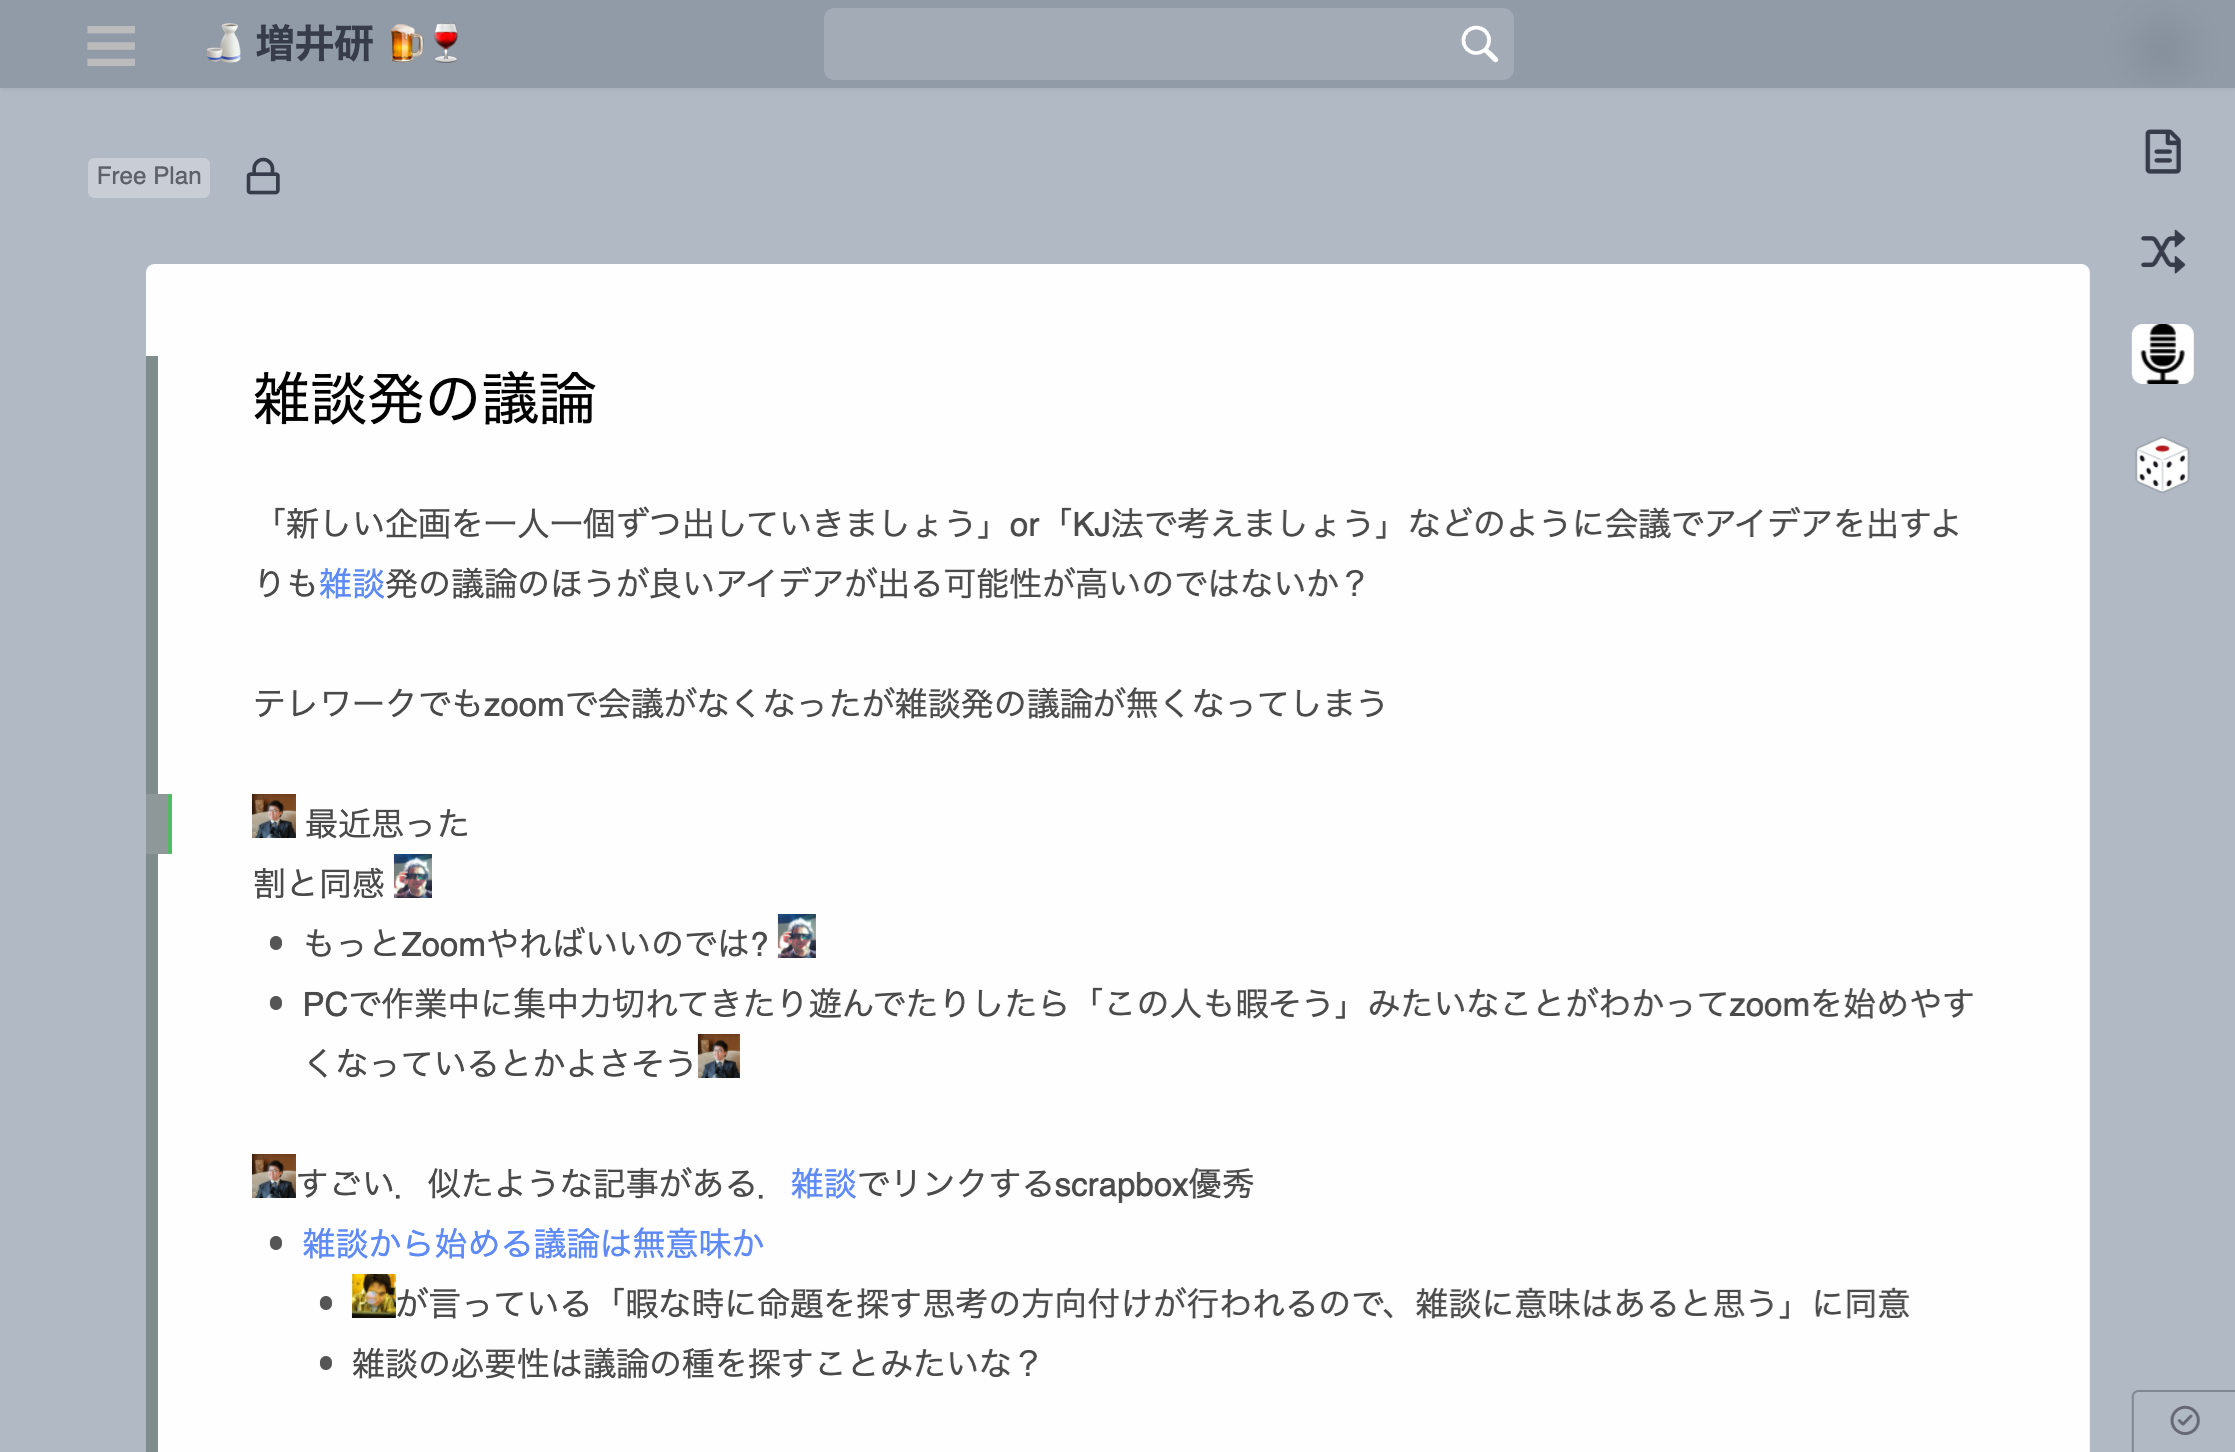
\includegraphics[width=9cm,bb=0 0 2235 1452]{figures/cca2e0eaed298ea4952a26d2effa238c.png}
  \caption{Scrapboxページ}
  \label{example1}
\end{figure}

リアルタイムにWikiを利用できるとアイデアの整理などにとても便利です。
様々なデータをカードに記録し、
それらを利用してアイデアをまとめるという手法が、
梅棹忠夫氏の「知的生産の技術」\footnote{
  \textsf{https:{\slash}{\slash}www.amazon.co.jp{\slash}dp{\slash}4004150930}
}や、
Niklas Luhmannによる
「Zettelkasten」\footnote{
  \textsf{https:{\slash}{\slash}en.wikipedia.org{\slash}wiki{\slash}Zettelkasten}
}などで提案され、広く利用されてきましたが、
これらは紙ベースのものでした。
ScrapboxはこれをWikiで実現したものであり、
柔軟で有用なシステムとなっています。

% https://the.kyoto/article/8035dca1-b561-4e01-ad81-4b5cc75161c1 から
\begin{figure}[t]
  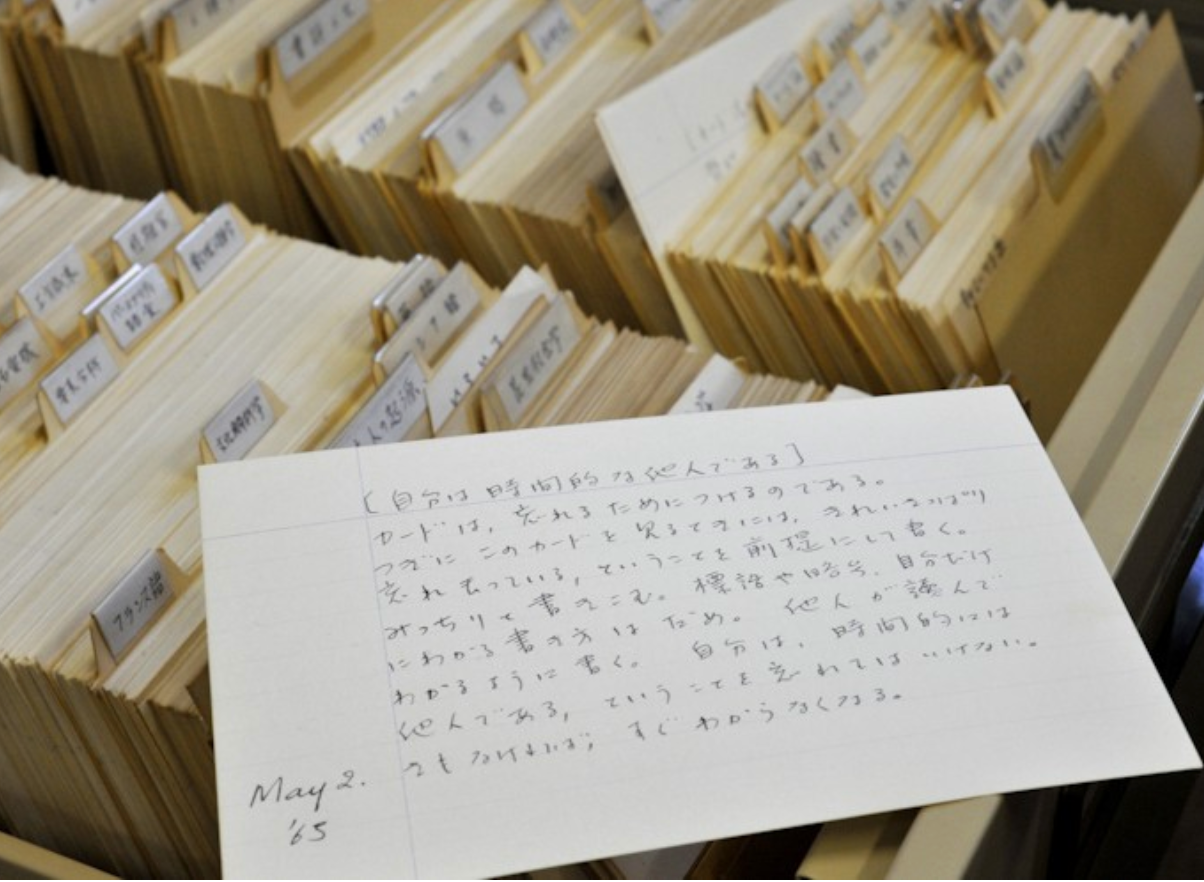
\includegraphics[width=9cm,bb=0 0 1204 882]{figures/1b2d14242e1eb302356a8f49c7450f04.png}
  \caption{梅棹忠夫氏の情報整理カード.}
  \label{umesaocards}
\end{figure}

\subsection{検索支援}

複雑なシステムやサービスが身のまわりに増えてきていますが、
使い方がわからないといった問題を解決することは簡単ではありません。
大抵のパソコンOSやアプリケーションにはヘルプ機能が用意されていますが、
ヘルプシステムを使って問題が解決できることは少ないため
活用されているとはいえず、
Webで検索したり他人に聞いたりすることで問題を解決してることがほとんどです。

\begin{figure}[t]
  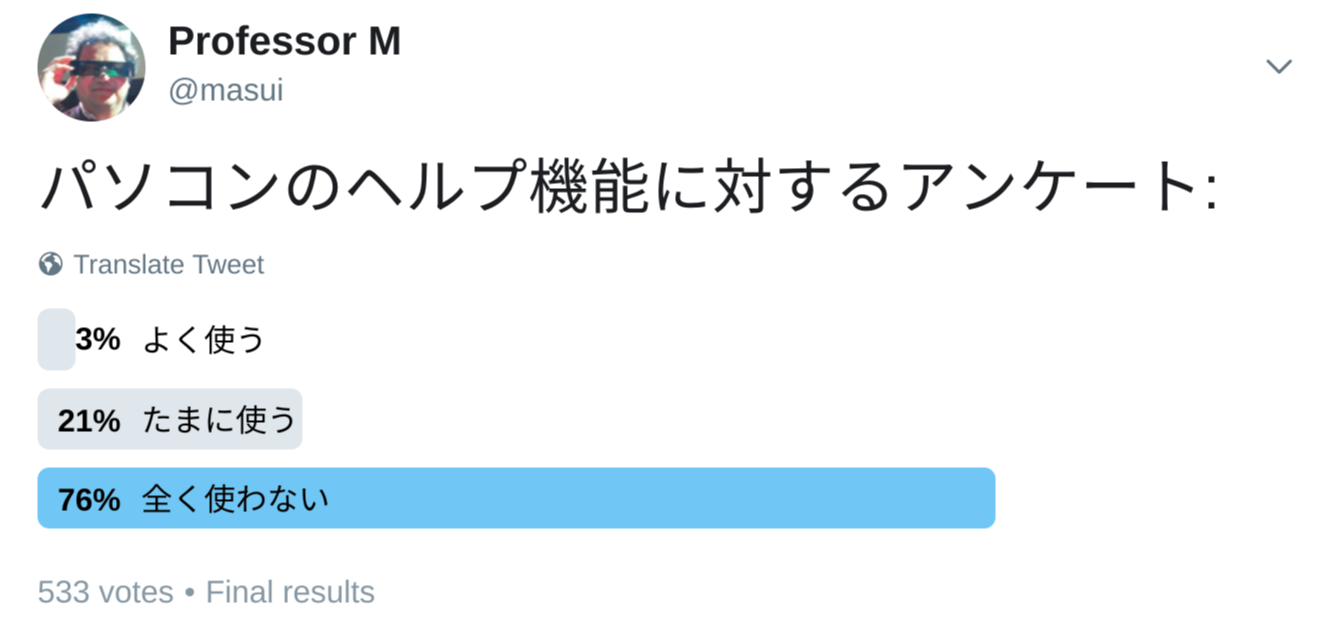
\includegraphics[width=10.3cm,bb=0 0 1332 623]{figures/383ee54c265ebbb88778d7ea0fbea5b1.png}
  \caption{ヘルプ機能の利用状況アンケート (2019/2/28)}
  \label{helpinquiry}
\end{figure}

ヘルプの検索にはキーワード検索が利用されるのが普通ですが、
ユーザの頭の中の単語とヘルプ文書中の単語は一致しないことが多いため、
必要な情報をうまくみつけるのは困難です\cite{10.1145/32206.32212}。
%
このような問題を解決するため、
頭の中に出現しそうなキーワードにマッチするあらゆるヘルプ文書を用意しておき、
キーワードと曖昧検索を行なうことによりヘルプを実現する
「展開ヘルプ」\cite{ExpandHelp}技術を開発し、
「Helpfeel」\footnote{
  textsf{https:{\slash}{\slash}helpfeel.com{\slash}}
}という商品名でサービスをしています。

図\ref{helpinquiry}は
Helpfeelでカラオケ店のサービスを検索しているところです。
検索キーワードの綴りが間違っていたり、
ドキュメントに含まれていないキーワードをユーザが指定した場合でも
適切なヘルプを表示できるようになっています。

\begin{figure}[t]
  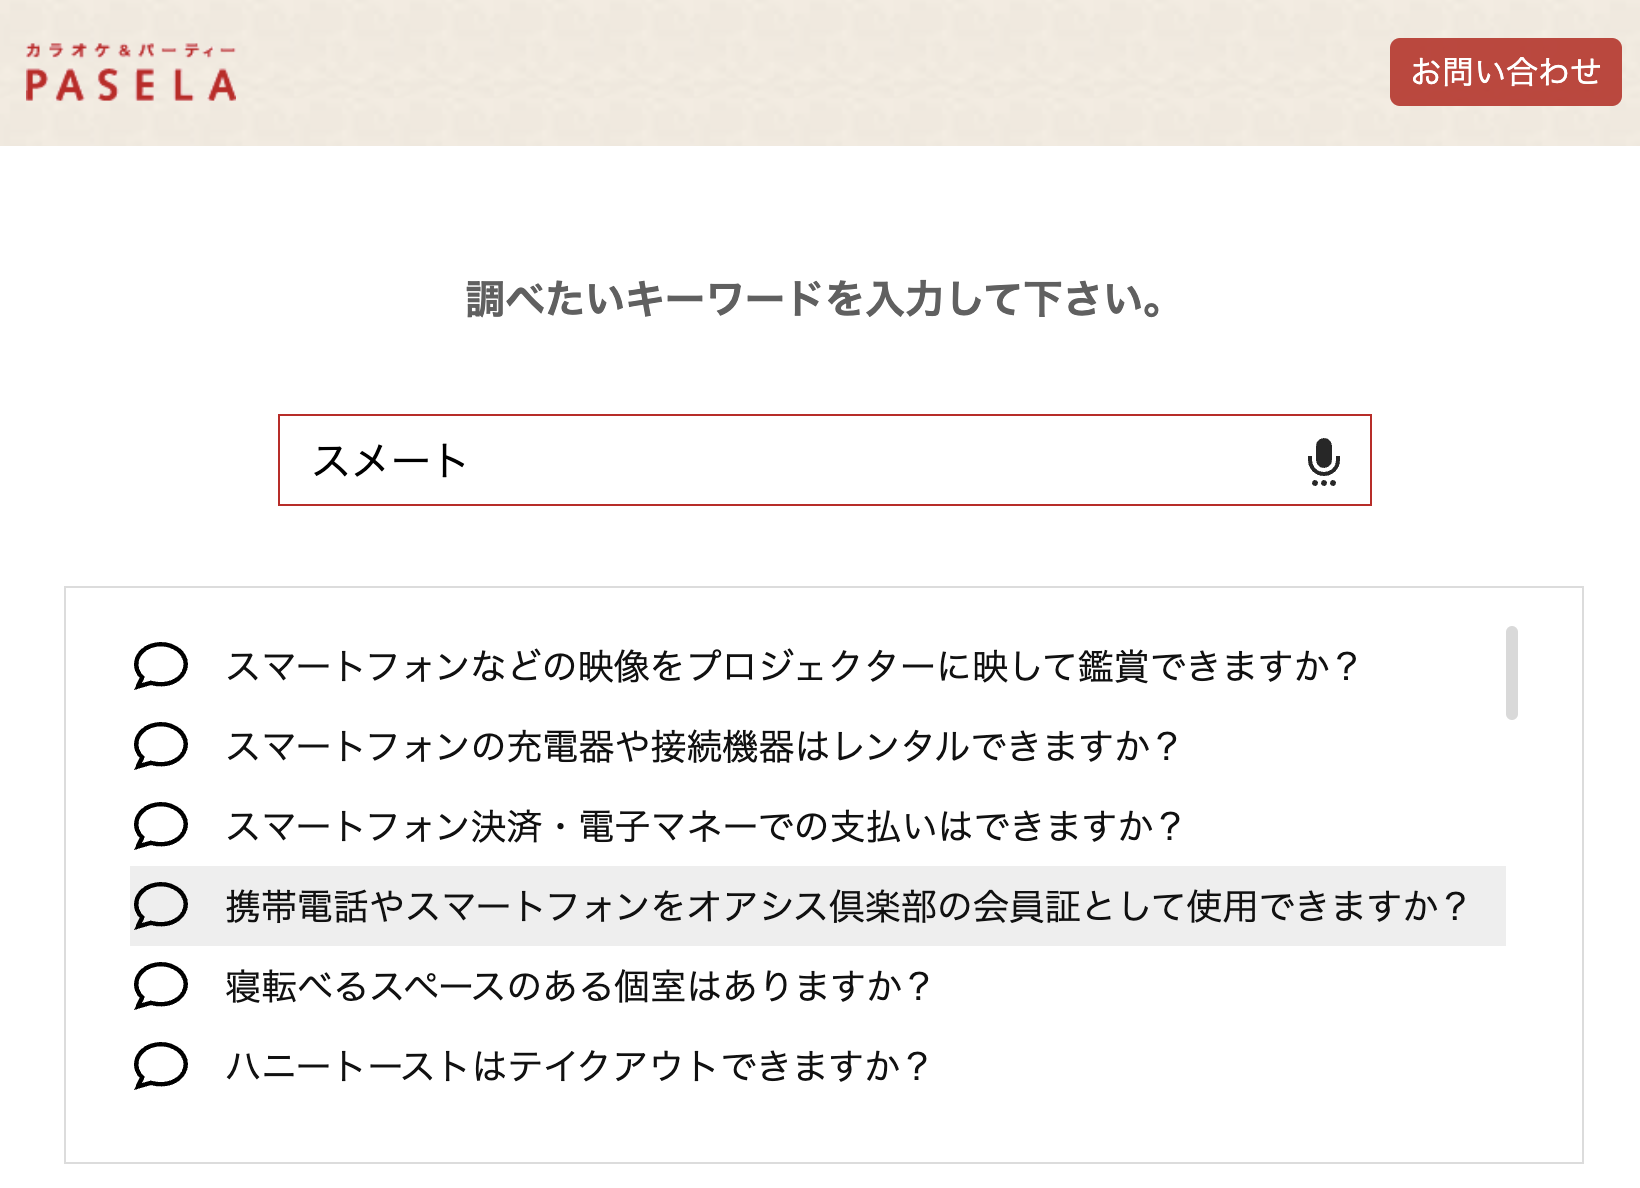
\includegraphics[width=10cm,bb=0 0 1640 1188]{figures/4b2ca6d18537ec8d6922e0389324c3ea.png}
  \caption{カラオケのヘルプ.}
  \label{helpinquiry}
\end{figure}

\subsection{コンテンツ閲覧}

ネットには大量のコンテンツが存在し、
パソコンやテレビ画面でそれらを楽しむことができますが、
コンテンツを選択するための操作は簡単ではないのが普通です。
パソコンの入力装置やリモコンのボタンを使って
目的のコンテンツを選択するためには
それなりのリテラシが必要です。

細かい選択操作が苦手な人でも、
最小限の操作でコンテンツを閲覧できるようにするため、
ふたつのキーだけを利用して大量のコンテンツを選択して楽しむことができる
「Serencast」\footnote{
  \textsf{http:{\slash}{\slash}Serencast.com{\slash}}
}システムを開発しました\cite{Serencast}。
Serencastを利用すると、
複雑なリモコン操作を全くせずに大量のコンテンツをブラウジングすることができます。

\begin{figure}[t]
  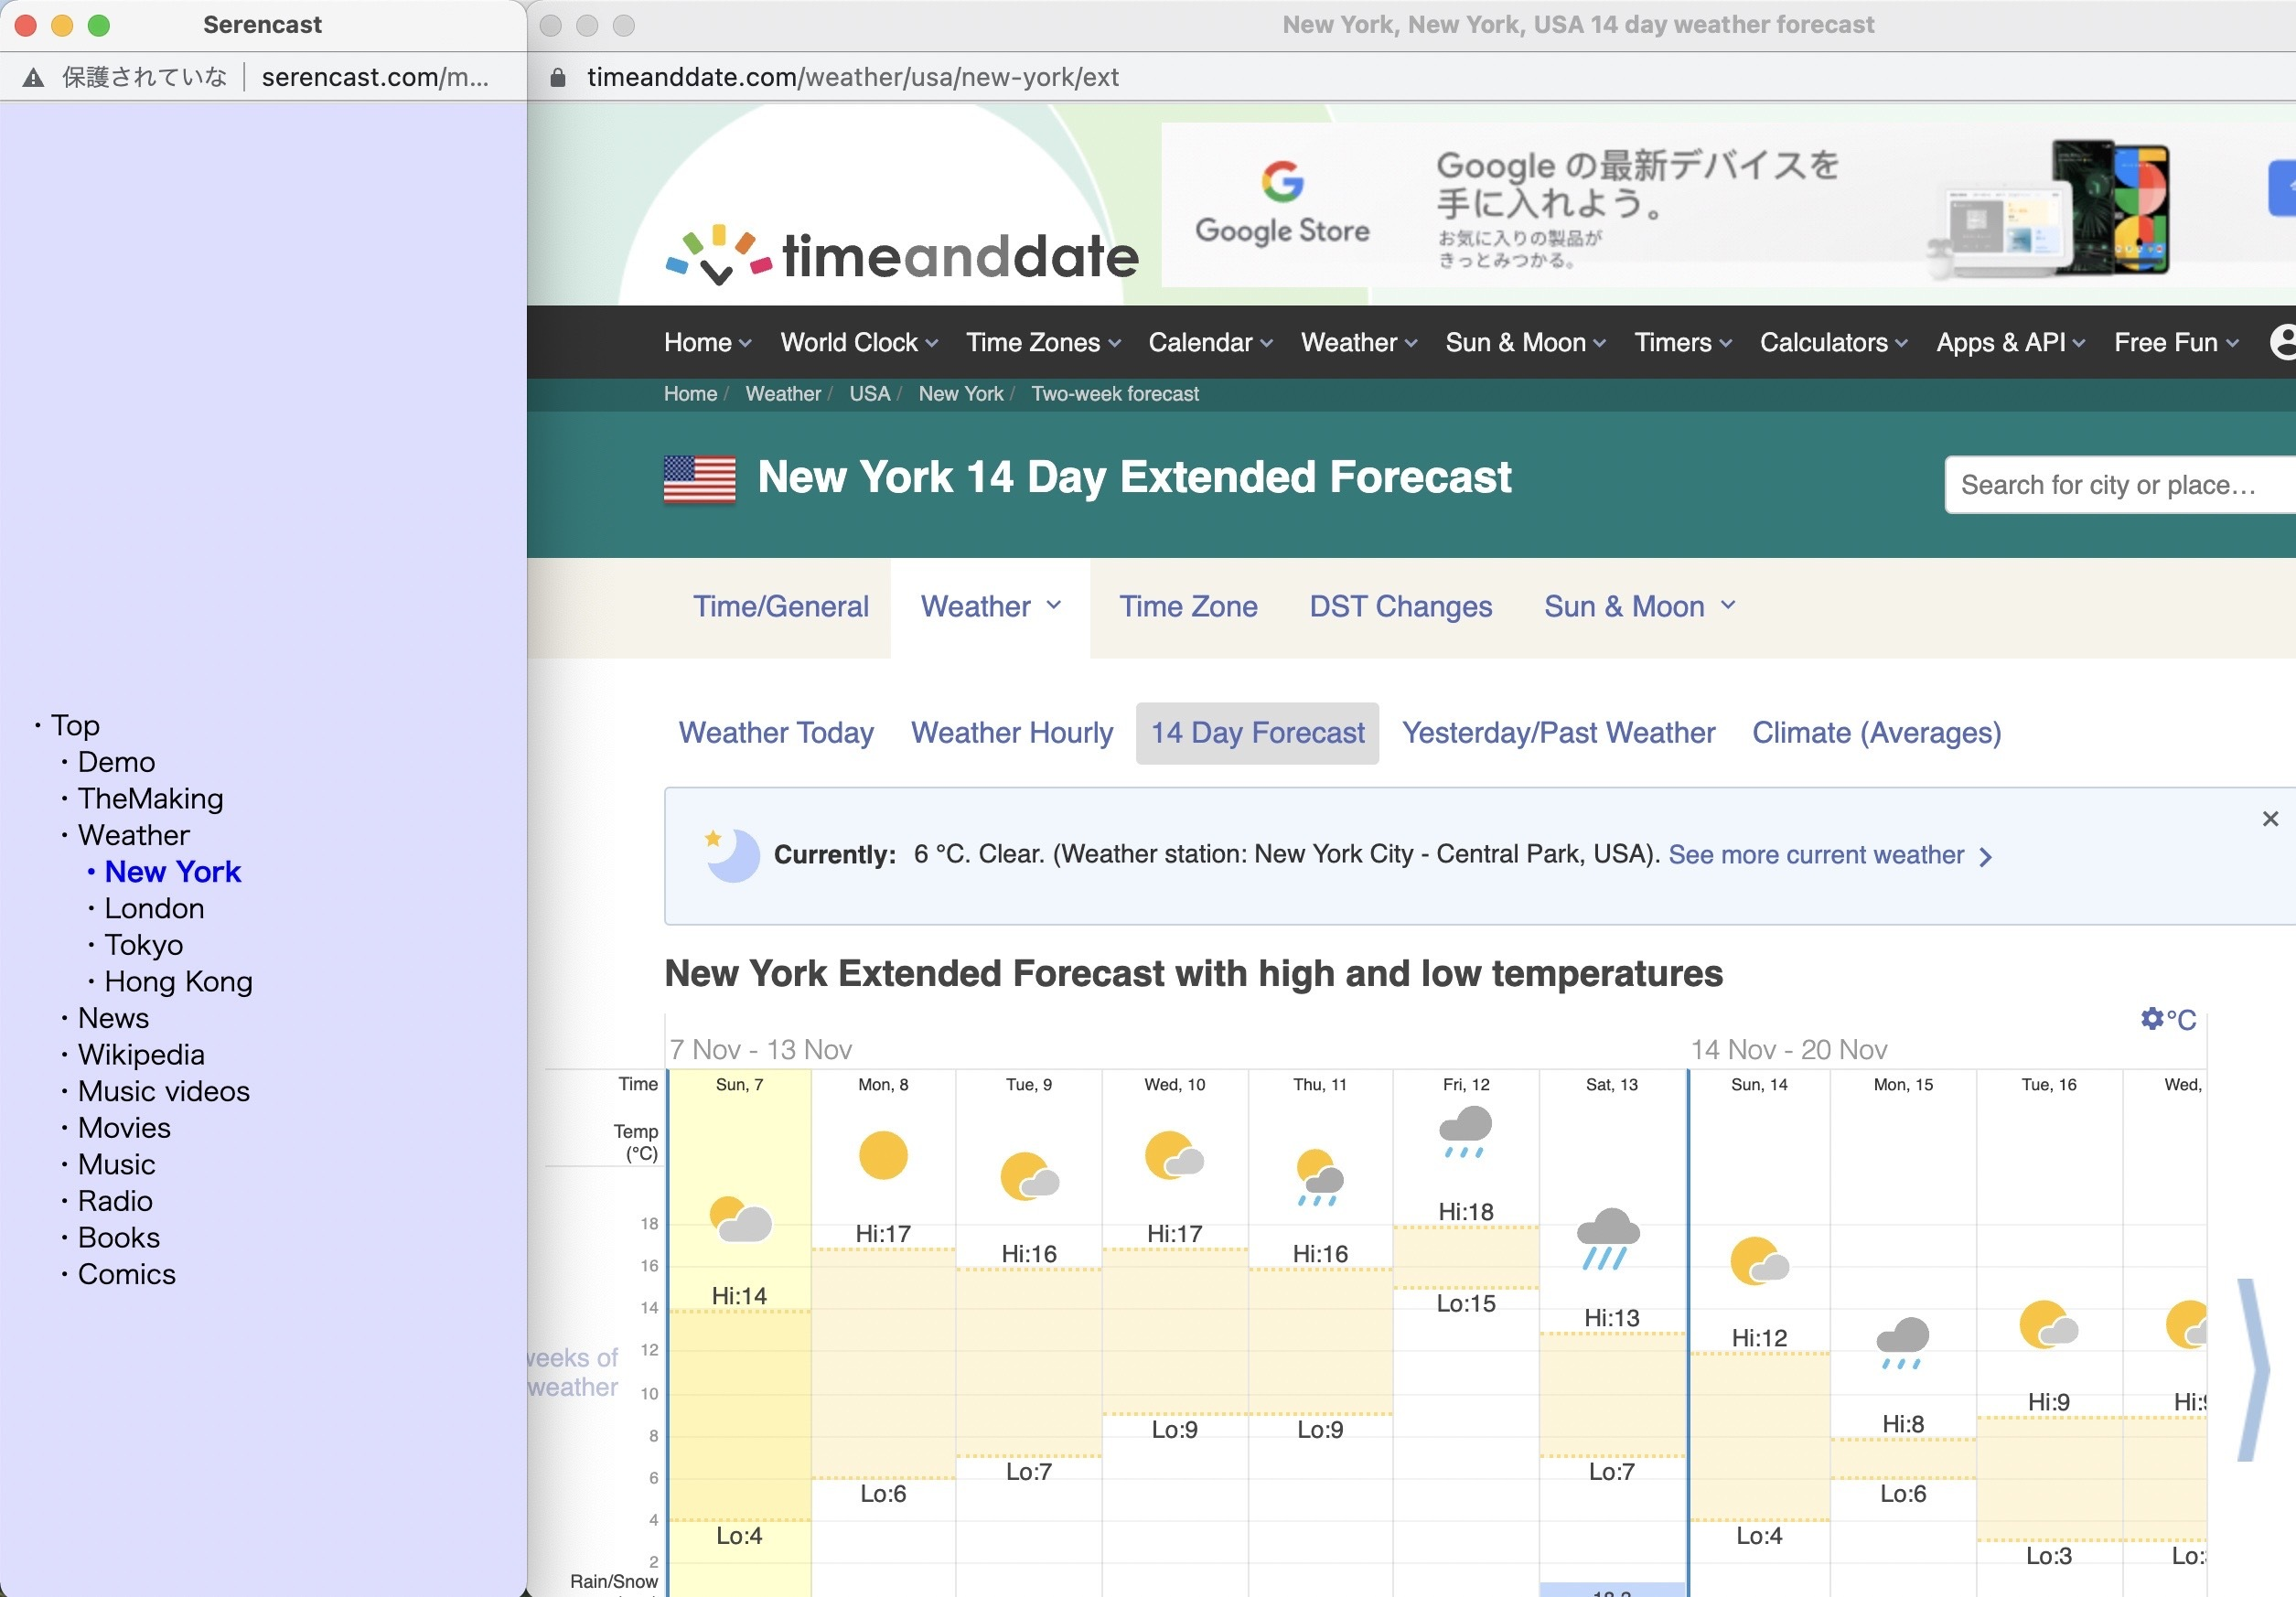
\includegraphics[width=9.5cm,bb=0 0 2510 1746]{figures/bb4027e2e210bc16450f0120a2987458.jpg}
  \caption{Serencastで天気予報を視聴.}
  \label{serencast}
\end{figure}

コンテンツは階層的なデータベースとして用意しておきます。
階層的データベースをナビゲーションするとき、
隣の情報に移動することに加え、
下の階層に移動するための操作や
上の階層に移動するための操作が必要なシステムがほとんどですが、
Serencastではこれらの移動が自動的に実行されるため、
最小限の入力装置でナビゲーションが可能になっています。

\subsection{パスワード管理}

ネット上のサービスを利用するとき、
パスワード漏洩の危険を避けるため、
サービスごとに異なるパスワードを利用することが推奨されています。
%
昔はパスワードが必要なシステムの数は多くなかったため、
パスワードは人間の頭で覚えることが前提でしたが、
沢山のサービスを利用することが普通になった現在、
サービスの数だけパスワードを覚えることは不可能です。

沢山のパスワードを利用するために
「パスワード管理システム」が広く利用されるようになってきましたが、
パスワード管理システムを利用するためには「マスターパスワード」が必要ですし、
特殊なパスワード管理システムはどこでも使えるとは限りません。

こういう問題を解決するため、
既に自分が覚えているエピソード記憶からパスワードを生成して利用できる
「EpisoPass」\footnote{
  \textsf{https:{\slash}{\slash}EpisoPass.com}
}というシステムを開発しました\cite{episopass2}\cite{episopass1}。
エピソード記憶とは、学習による「意味記憶」と異なり、
体験にもとづいて覚えていて忘れることが少ない記憶のことです。
EpisoPassでは、
自分だけが覚えているエピソード記憶を問題として登録しておき、
答の候補の中から正答を選択します。
答の選択によって異なる文字列が生成されますが、
正しい答を選択したときに生成される文字列をパスワードとして登録します。
問題と答候補の組を保存しておけばパスワードをどこでも生成できるので、
マスターパスワードのようなものは必要ありませんし、
パスワードを忘れてしまう心配がありません。

\begin{figure}[t]
  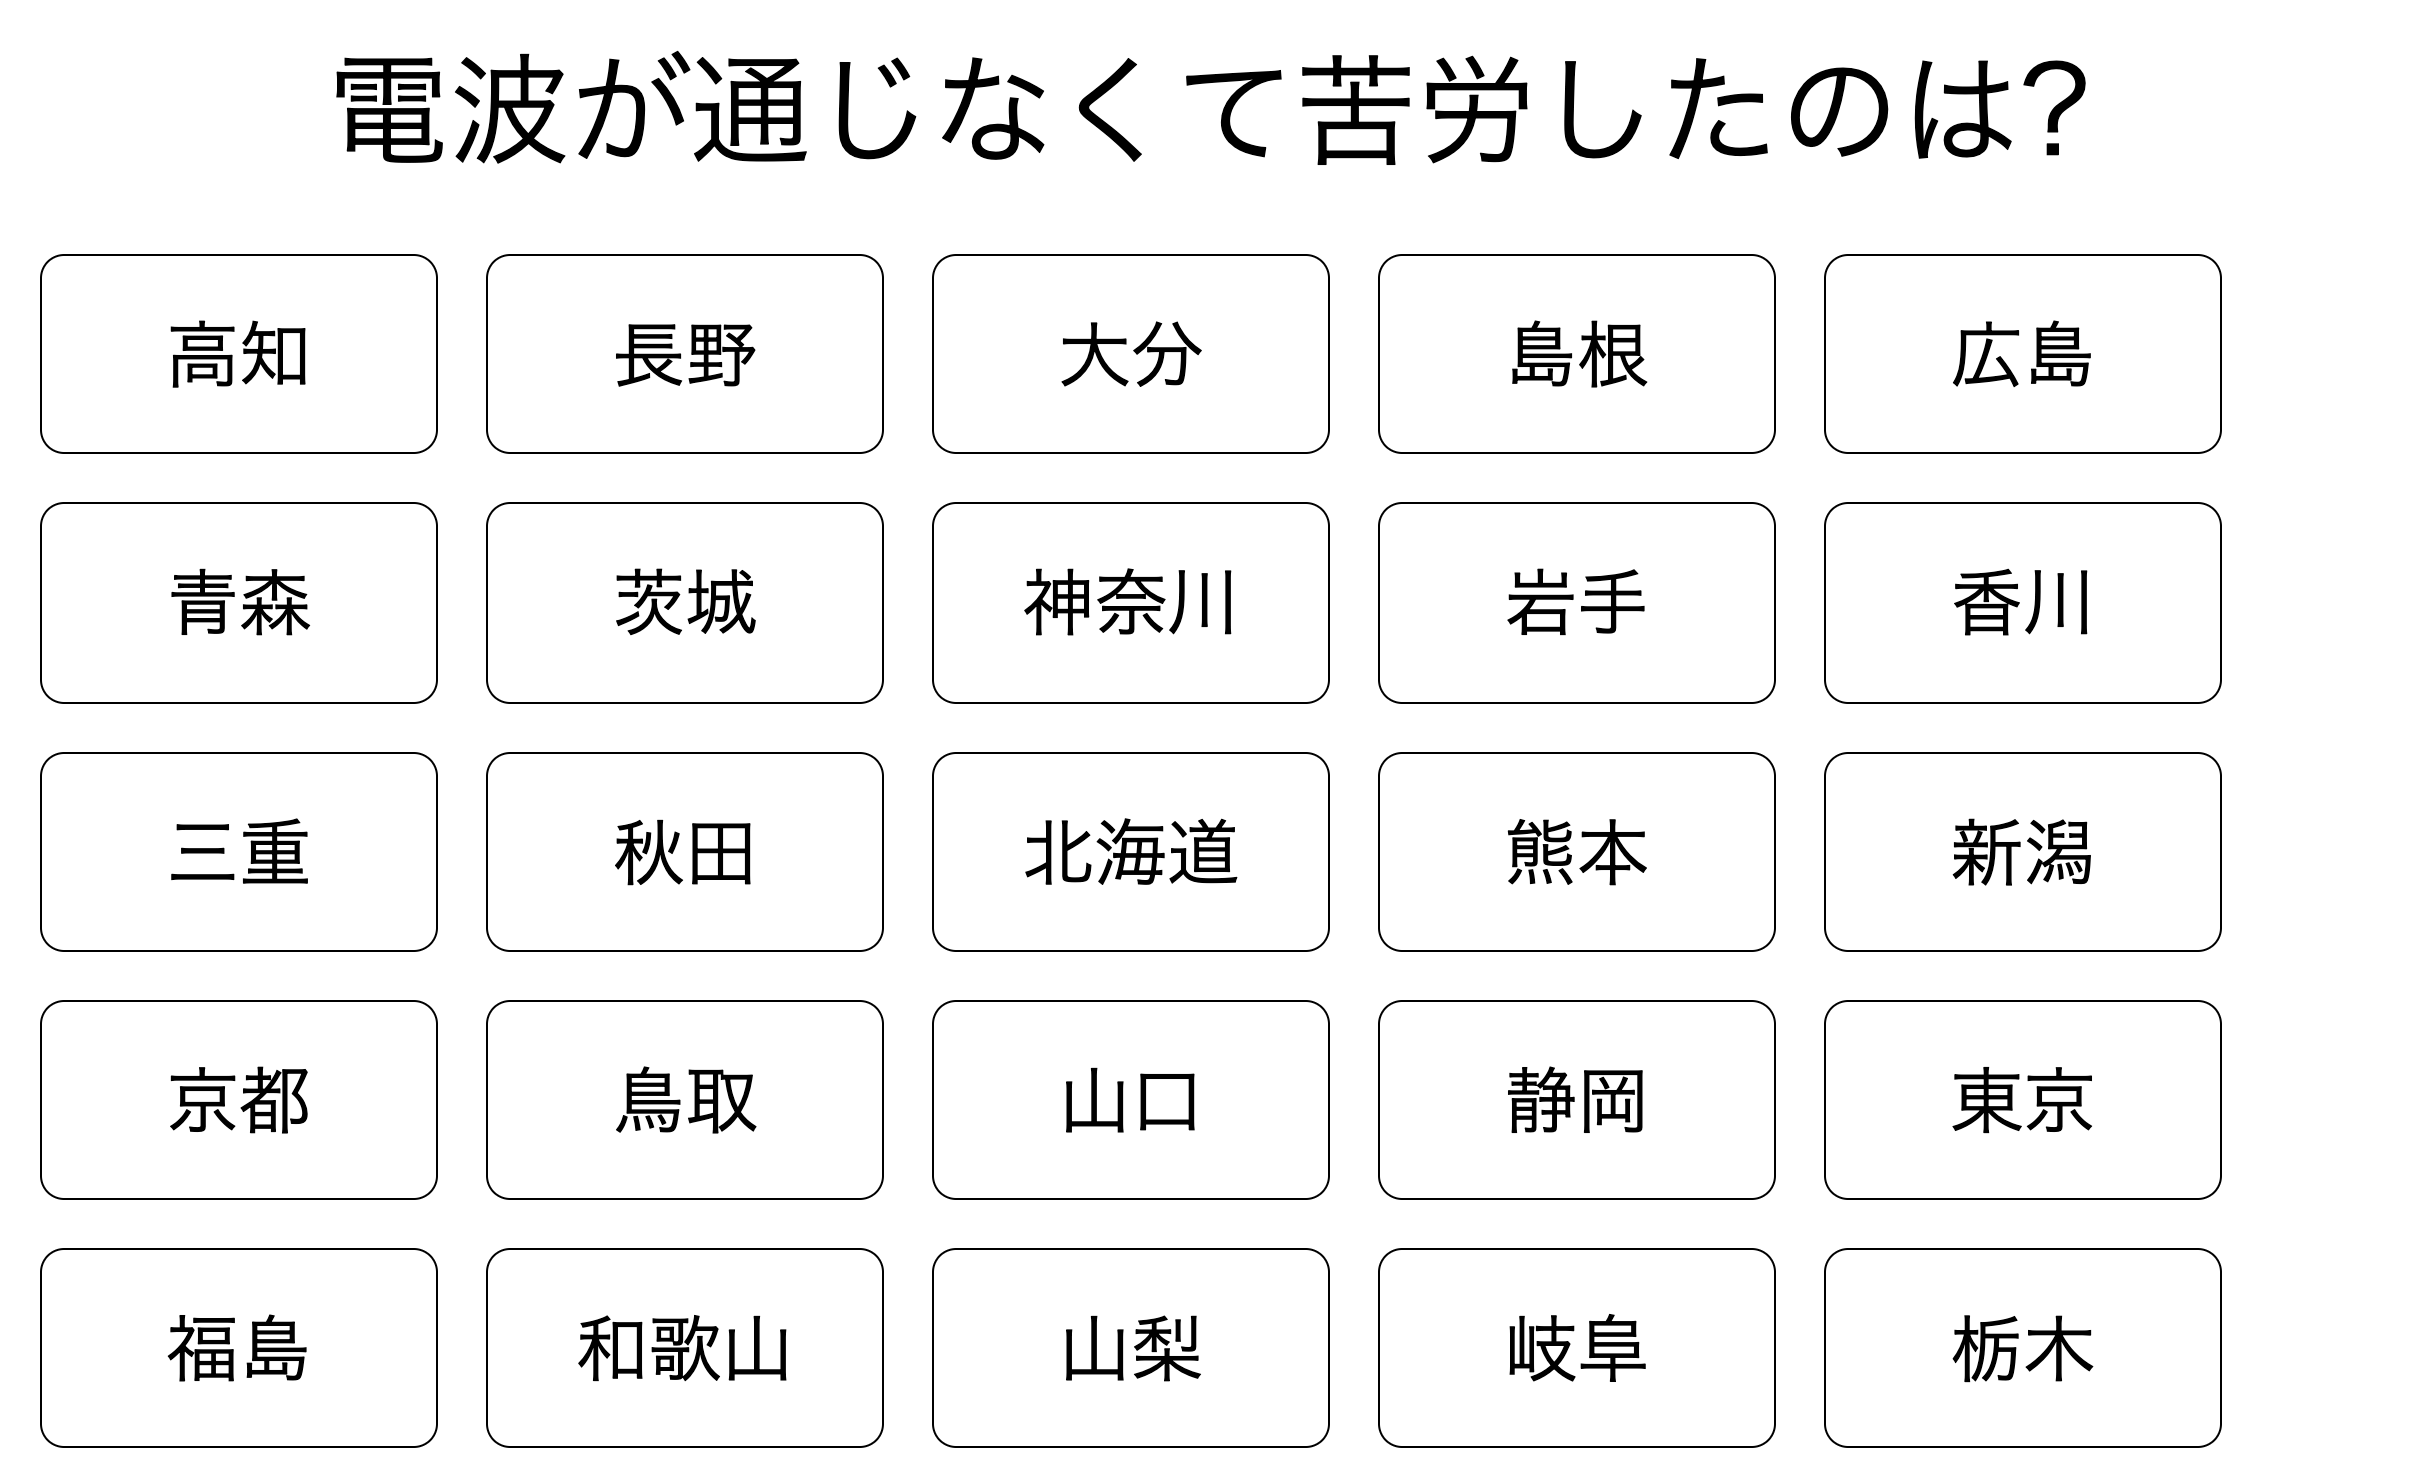
\includegraphics[width=10.2cm,bb=0 0 2418 1480]{figures/e5c3cabfe3011ef807b5e045c2d83ea8.png}
  \caption{EpisoPass問題.}
  \label{episopass}
\end{figure}

パスワード管理システムの利用法やマスターパスワードを覚えておくことには
リテラシが必要ですが、EpisoPassでは特別に記憶しなければならないことが無いので、
ユニバーサルに利用できるシステムだといえるでしょう。

\section{まとめ}

長年にわたり、誰もがいつでもどこでも利用できる
ユニバーサルなアプリケーションやサービスの開発に勤めてきました。
有用なアプリケーションを作成するためには
基礎的なコンピュータサイエンスの技術が必要です。
コンピュータソフトウェアの知見にもとづき、
ユニバーサルなインタフェースをさらに開発していきたいと考えています。

\bibliographystyle{jssst}
\bibliography{paper}

\vspace{2mm}

% \newif\ifChoshaPicture \ChoshaPictureTrue
\def\choshapicturex#1{%
  \vbox to 8mm{\hbox to 20mm{\includegraphics[width=28mm,bb=0 0 986 1186]{#1}}}}
\choshapicturex{figures/f91ce16aa949ec47fa99da1fe7809b88.jpg}

\chosha{増井俊之}{
  1984年東京大学大学院工学系研究科電子工学専門課程修士課程修了。 工学博士。
  シャープ、ソニーコンピュータサイエンス研究所、産業技術総合研究所、Apple Inc.などに勤務後、
  2009年4月より慶應義塾大学環境情報学部教授。
  情報検索、テキスト入力、情報視覚化、実世界指向インタフェース、予測インタフェース、認証技術など、
  ユーザインタフェースに関連する幅広い研究開発を行なっている。
  携帯電話やスマートフォンで広く利用されている予測入力システムPOBoxや
  フリック入力システムの開発者。
  Gyazo, Scrapbox, Helpfeel, EpisoPass, 本棚.orgなど
  各種のWebサービスを運用中。
  }
  
\end{document}

% https://scrapbox.io/masui/%E3%82%BD%E3%83%95%E3%83%88%E3%82%A6%E3%82%A7%E3%82%A2%E7%A7%91%E5%AD%A6%E4%BC%9A_%E5%9F%BA%E7%A4%8E%E7%A0%94%E7%A9%B6%E8%B3%9E%E8%AC%9B%E6%BC%94
